% Superseded by evaluation-questions.tex; retained as historical source, not compiled.
\section{Benchmarks, capacity and reproducibility}
\label{sec:evaluation}
\subsection{Two kinds of evidence}
This revision includes fresh local scaling measurements as well as historical
performance records. Tests establish outputs, gradients and guards for explicit
cases. Archived timings describe the recorded implementation and environment;
rerendering a figure is not rerunning an experiment. Some old records lack full
source revision, seed or environment metadata. Attaching the current environment
does not repair that missing provenance.

The implementation archive contains 50 hashed JSON inputs, including 44 registered
benchmark cases and supporting measurements. The documentation publishes an input
index and a downloadable archive. Plot generators preserve the provider, phase,
shape, precision and cache-state boundaries. A ratio is defined by
$$
 \text{speedup}=\frac{\text{matched baseline latency}}{\text{candidate latency}}.
$$
Ratios below one indicate a slower candidate. Different topology, feature width,
precision, output semantics or build/reuse scope cannot be silently grouped as
one comparison. Median latency, sampling confidence interval, correctness checks
and release readiness are separate facts.

\subsection{Fresh experiment setup and questions}
The September 19 experiments address (Q1) forward latency versus graph size on
the ordinary Torch input path, (Q2) executable capacity under controlled native
allocation budgets, and (Q3) billion-edge execution when a full working set
exceeds physical GPU capacity. The host has an AMD Ryzen 7 255 (8 cores, 16 logical
CPUs), about 44 GiB of RAM and an NVIDIA RTX 5070 Ti with 16 GiB device memory.
The GPU driver is 595.84, Torch is 2.11.0+cu128 and Triton is 3.6.0. Runs use a
local dirty checkout, not an immutable release. Command lines, dependency
versions, timestamps, source-diff hashes and untracked-source hashes accompany
the data. This was not a dedicated, clock-locked benchmark machine; intervals
describe within-run sampling, not reproducibility across hosts.

The GPU sweep contains 8,192, 32,768, 131,072 and 524,288 nodes, at feature widths
16 and 64. Each row has a seeded degree uniformly selected from 8 through 24,
with random source IDs, FP32 weights/features and int32 CSR indices. Duplicate
edges are retained. The fixed seed is 20260919. All three implementations receive
the same graph and values; topology construction, CSR wrapper creation and index
conversion are outside timing. Inputs do not require gradients.

Five warmup calls precede 20 CUDA-event samples per implementation and
configuration, with provider order randomized each round. Outputs are checked
against an explicit gather--multiply--scatter oracle at relative and absolute
tolerances of $3\cdot10^{-4}$ before timing. The public ordinary Tiga call is
measured, not prepared execution. Diagnostics record a compiler-emitted bounded
ragged weighted-sum route. First-call host wall time is retained separately;
the warm curves exclude first compilation, transfers and backward. CUDA events
may include device idle time between host submissions; these are not isolated
instruction-throughput measurements.

\begin{figure}[htbp]
\centering
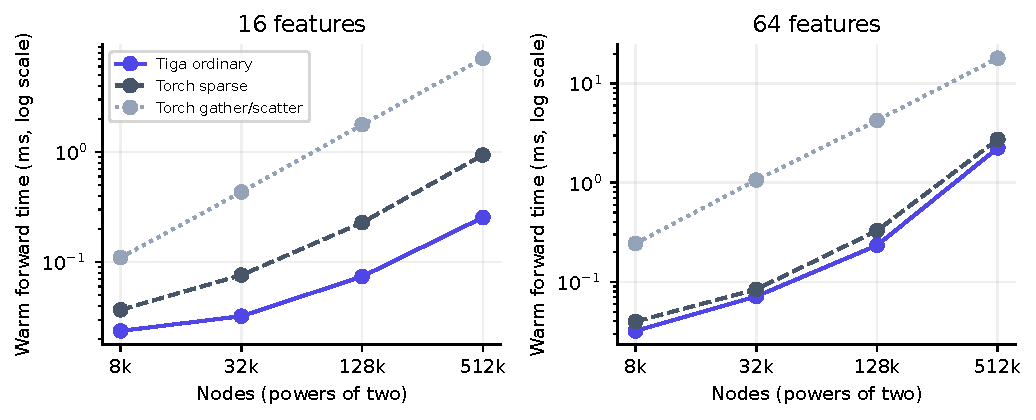
\includegraphics[width=\linewidth]{figures/gpu-latency.pdf}
\caption{Fresh ordinary-Torch forward latency on the RTX 5070 Ti. Both panels
use the same graph-size sweep; feature widths remain separate. Lower is better.
The logarithmic time axes expose both small and large workloads.}
\label{fig:gpu-latency}
\end{figure}

\begin{figure}[htbp]
\centering
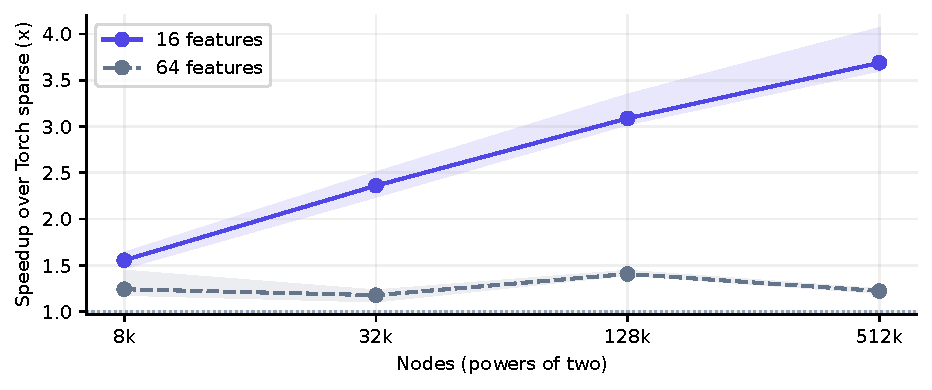
\includegraphics[width=.9\linewidth]{figures/gpu-speedup.pdf}
\caption{Fresh Tiga ordinary-call speedup against the fixed Torch sparse peer.
The dotted line is parity. Shading is a pointwise 95\% paired bootstrap interval
of the median-latency ratio (5,000 resamples of the 20 interleaved rounds,
seed 20260919), not a cross-machine confidence claim.}
\label{fig:gpu-speedup}
\end{figure}

Figures~\ref{fig:gpu-latency}--\ref{fig:gpu-speedup} expose the dependence on
graph size and feature width rather than collapsing all shapes into a single
number. Across these four sizes, the median-latency ratio against Torch sparse
ranges from 1.56 to 3.69 at width 16 and from 1.18 to 1.41 at width 64.
These ranges describe the measured points, not a bound for arbitrary graphs.
The gather--scatter baseline is deliberately labeled as one
implementation; the sparse-library baseline is also shown. These are forward
operator results, not end-to-end training, generalized PyG performance or
compiled-backward speedups. The full numerical samples and per-case dispatch
diagnostics are included in \code{data/gpu-scaling.json}.
\FloatBarrier

\subsection{Capacity under an 8 MiB native RAM budget}
The CPU experiment uses a periodic one-dimensional graph with 16 source-neighbor
offsets per destination and a scalar source field $x_i=i\bmod97$. Each output is
the mean of its 16 neighbors. This is a controlled regular-local graph, not a
power-law dataset or an irregular-feature IO stress test. The topology and source
field are persisted before execution. Ingest is outside the question of
executing an existing stored graph and is not included in the curves.

Three execution choices are compared: full materialization through the public
API, paging 1,024 destination rows, and paging 8,192 rows. Prefetch is disabled to
isolate the page-size/capacity tradeoff. All use the same 8 MiB \emph{native-buffer}
budget. Each of three trials runs in a fresh process and performs one forward
evaluation. Time includes loading the chosen representation and its first
execution, including needed JIT work; process startup, ingest and the independent
NumPy oracle are excluded. Repeated unchanged-input calls are deliberately not
used as an execution-latency proxy for the lazy native path. The OS page cache
is not forcibly cleared, so this is not a cold-NVMe bandwidth experiment.

Every completed output is compared elementwise against an independently computed
periodic-stencil oracle; all successful trials have zero maximum absolute error.
The output remains resident, so paging does not make memory independent of
node count. Disk-backed field handles, bounded staging, output assembly,
Python/compiler allocations and OS file caching have distinct accounting rules.

\begin{figure}[htbp]
\centering
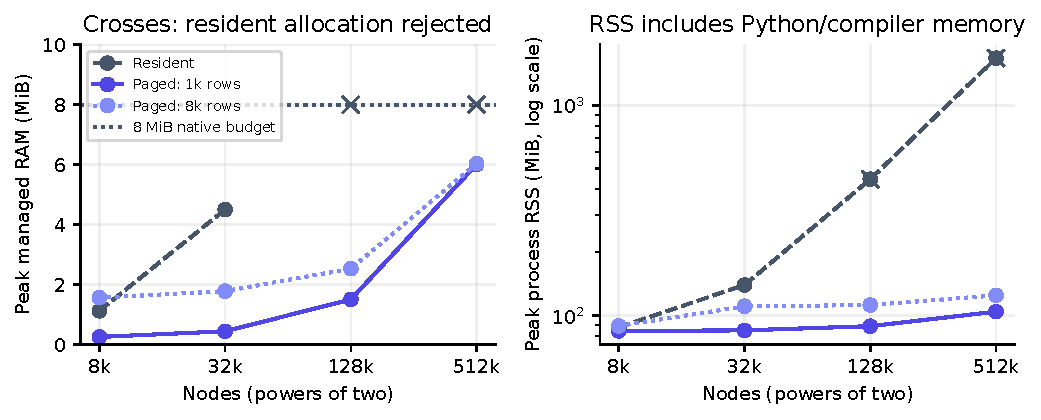
\includegraphics[width=\linewidth]{figures/memory-capacity.pdf}
\caption{Fresh CPU capacity experiment. Left: maximum tracked RAM across three
fresh processes, with the 8 MiB native budget. Crosses mark rejected resident
configurations, not measured allocations of exactly 8 MiB. Right: maximum
process RSS, including rejected materialization attempts. RSS is not limited
by the native budget.}
\label{fig:memory-capacity}
\end{figure}

\begin{figure}[htbp]
\centering
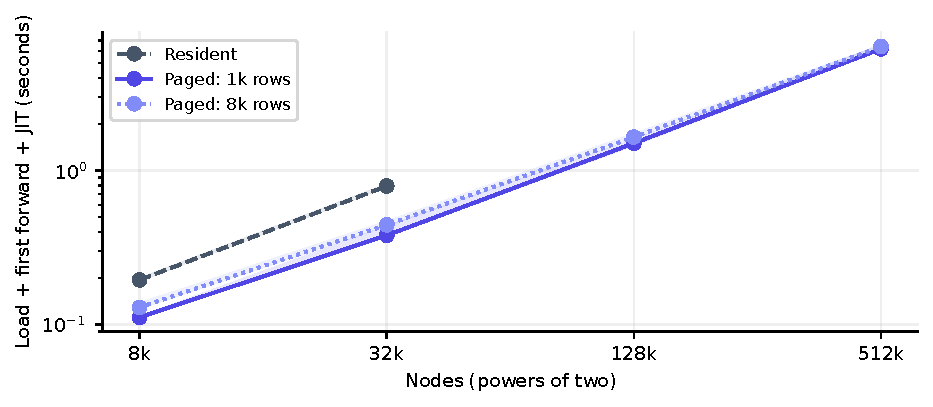
\includegraphics[width=.9\linewidth]{figures/memory-time.pdf}
\caption{Load plus first forward execution, including JIT, on CPU. Lines show
the median of three fresh processes and shading the observed minimum--maximum
range. Missing resident points are budget rejection, not zero latency.}
\label{fig:memory-time}
\end{figure}

At 131,072 nodes the resident path is rejected while both paging choices finish.
At 524,288 nodes (8,388,608 edges), the stored topology and field occupy about
70 MiB, but paging completes under the 8 MiB native budget. The 1k-row and
8k-row choices peak at approximately 6.01 and 6.03 MiB of tracked native RAM;
maximum process RSS is approximately 104.5 and 124.9 MiB. Their median load-plus-
first-execution times are about 6.18 and 6.40 seconds, respectively. Thus the
capacity result is not ``a graph ran using only 8 MiB of total machine memory.''

The rejected resident materialization at the largest size still reaches about
1.63 GiB RSS because Python index materialization precedes the managed native
allocation check. This is a concrete limitation of the current loader and
accounting boundary, not evidence of a hard process-memory cap. The relative
first-execution times at smaller sizes also include loading and JIT differences;
they cannot be relabeled steady-state kernel speedups. The useful result is that
paging extends the executable graph range under the stated resource policy.

This earlier CPU experiment does not establish GPU-to-NVMe streaming, graphs larger
than host physical RAM, a byte-budget-derived automatic page-size optimizer,
training throughput, or arbitrary repeated multi-step execution at this budget.
Those require separate sweeps with physical resource enforcement, IO statistics,
graph skew, feature width, backward state and sustained iterations. This
single-invocation CPU experiment does not establish iterative execution support.
The following experiments measure two-host execution and a separate ten-step
CUDA paging workload, with their own configurations and source records.
\FloatBarrier

% Historical TCP evaluation, superseded by the NCCL experiment; not compiled.
\subsection{Heterogeneous two-host execution}
\label{sec:two-host}
The next experiment uses both available GPUs: the RTX 5070 Ti Linux host and
an RTX 4070 Ti SUPER (16 GiB) under Ubuntu/WSL on a second Windows host. They
communicate over the private network using TCP host staging. Both retain their
existing service workloads; about 3 GiB and 10--11 GiB of GPU memory were already
occupied. This is not a same-host NVLink/PCIe experiment or a dedicated cluster.
Both rank records contain matching hashes for every Tiga Python source and both
compiler executables. Environment and driver versions are retained per rank.

The graph has 16 edges per row and 16 FP32 features. Destination ownership is
split equally. Three quarters of the rows gather within their owner's half;
every fourth row gathers 16 neighbors from the other half. Overlapping remote
neighborhoods make the required ghost set large: boundary-row fraction alone
is not the exchanged-byte fraction. The sizes are 8,192, 32,768 and 131,072 nodes.
Each GPU also runs the complete graph alone with identical values and semantics.
This is strong scaling of one fixed graph, not doubling the graph with the ranks.
Topology is replicated for setup on both hosts and its partition maps are cached;
runtime source fields contain only owned rows before halo exchange. This is not
evidence that the topology itself was distributed beyond one device's capacity.

Each configuration has three warmups and ten measured calls with changed input
scales. Every output is checked against an independent NumPy construction of
the global result. Timings are synchronized host-wall intervals through output
completion, excluding graph/input creation, an inter-rank control barrier and
oracle checking. The distributed critical path is the maximum of the paired
rank durations for each round; it is not the average of two ranks. The methods
run in a fixed order, so drift and other host workloads remain confounders.
These native-input host-wall measurements are not interchangeable with the
earlier ordinary-Torch CUDA-event measurements.

\begin{figure}[htbp]
\centering
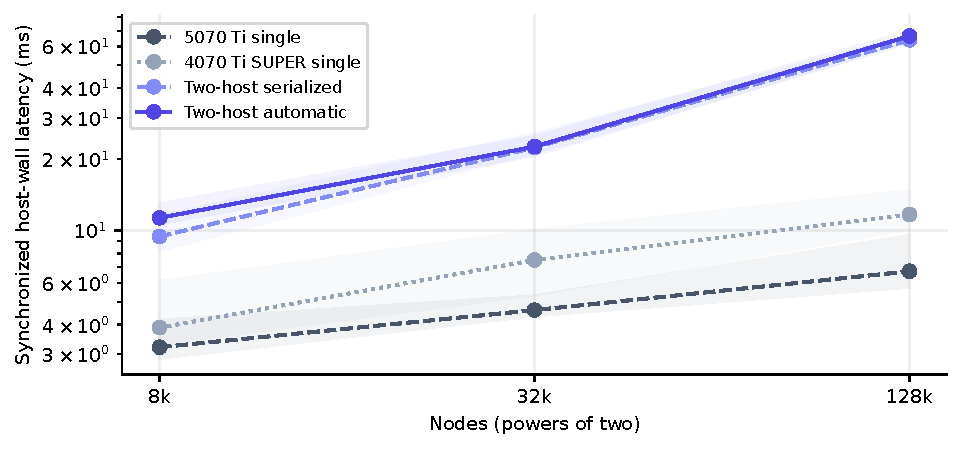
\includegraphics[width=.94\linewidth]{figures/two-host-latency.pdf}
\caption{Real two-host TCP scaling versus each GPU running the complete graph.
Lines are medians; bands show sample minima and maxima. Lower is better.
This configuration provides no multi-GPU speedup.}
\label{fig:two-host}
\end{figure}

At 131,072 nodes, the 5070 Ti and 4070 Ti SUPER single-GPU medians are 6.72 and
11.68 ms. Two-host serialized execution takes 64.00 ms and the automatic path
66.46 ms on the paired critical-path definition. At the smallest size the
automatic path is also slower than serialization (11.31 versus 9.44 ms).
Correctness and execution on two devices therefore do not establish useful
scaling. Automatically creating interior/boundary work is not a successful
cost model for deciding when its extra launches and assembly pay off.

\begin{figure}[htbp]
\centering
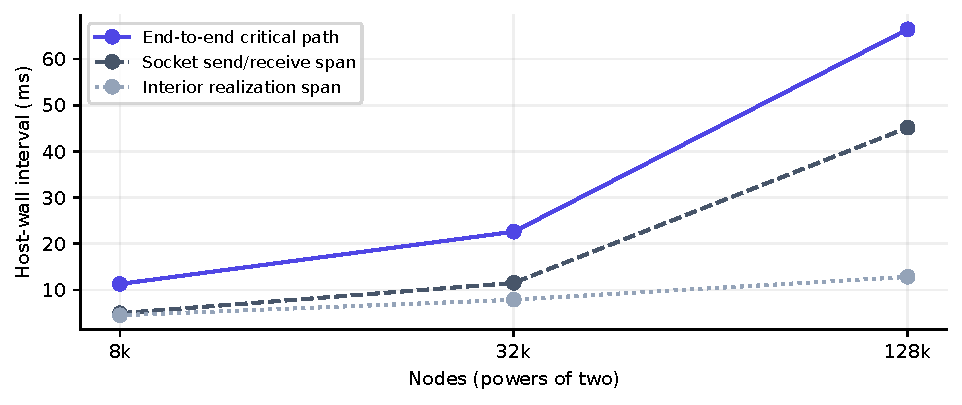
\includegraphics[width=.94\linewidth]{figures/two-host-components.pdf}
\caption{Host intervals in the automatic two-host run. Socket span covers the
first send/receive entry through the last return, including waits; it excludes
some packing, device copies and assembly. Interior realization includes host
submission. These intervals can overlap and must not be stacked or added as
exclusive components; they are not GPU-profiler measurements.}
\end{figure}

The raw records include sent/received payload bytes and per-rank interval traces.
The observed costs motivate reducing host staging, Python packing and repeated
assembly, and evaluating transport-aware scheduling. They do not prove that a
different transport or partition would deliver a particular speedup.

The NCCL configuration connects the two hosts through an isolated WireGuard
interface with bidirectional private addresses and MTU 1200. This fits the
WSL host's 1280-byte outer-interface MTU without changing the default route.

Both machines then passed a checked bidirectional 1 MiB exchange with the same
NCCL 2.28.9 library hash. A separate eight-node ring graph also passed forward
and source-VJP checks on both GPUs, in serialized and automatic schedules and
with changed inputs. The automatic trace reports two interior and two boundary
rows per rank; doubled input scale doubles the expected gradient from 3 to 6.
The runtime uses NCCL's device-buffer interface, but NCCL selects its Socket
network plugin over the encrypted tunnel, not GPUDirect RDMA. These are
correctness gates, not a bandwidth benchmark, scaling curve or device-profiler
proof of useful overlap. Earlier TCP timing curves are unchanged. Commands,
library/source hashes and both ranks' results accompany the report in
\code{data/runtime/}.
\FloatBarrier

% Original capacity discussion; data reused in evaluation-questions.tex. Not compiled.
\subsection{Billion-edge execution on a 16 GiB GPU}
\label{sec:gpu-paging}
The capacity experiment evaluates a graph whose full resident working set
exceeds the GPU's physical memory. The largest configuration contains exactly
one billion directed edges, 62.5 million nodes and 32 FP32 source features.
Every destination gathers its next 16 neighbors on a periodic ring and computes
their mean. The explicit CSR uses 64-bit indices; all edges are stored and
traversed, without replacing message passing by an analytic stencil kernel.
This regular-local topology isolates capacity and streaming costs; it does not
represent random power-law gathers.

The CSR occupies 8.50 GB and the source and output fields occupy 8.00 GB each.
Their combined resident lower bound is 24.50 GB (22.82 GiB), before scratch
buffers or compiler allocations. Thus full residency exceeds a 16 GiB device
even without other services. This is a lower-bound capacity comparison, not
an observed out-of-memory timing and not a claim that every alternative sparse
implementation requires these bytes: narrower indices or compressed relations
can change the footprint. Even with 32-bit CSR indices, the same source and
output fields give an 18.86 GiB lower bound, still above device capacity.

The fixture writer emits bounded chunks into the versioned CSR store and
records hashes of all three payloads. The public loader opens metadata-only
field handles. Execution streams 65,536 destination rows at a time, gathers
source values into host staging, copies the page to CUDA, and lowers FP32 CSR
sum to a bounded per-row reduction. Completed pages are written into the final
resident output through a single reusable-size host payload. The 7.45 GiB
output must fit device memory; the full input need not be resident there.
Each worker has a 12 GiB native-allocation safety budget, reduced if needed to
leave 512 MiB of currently free device memory uncommitted. Existing services
occupy about 3 GiB. The capacity comparison uses the physical device size,
not this software budget.

Each trial runs one forward in a fresh process. Time includes JIT lookup or
compilation, page reads, host/device copies, computation and output assembly.
Fixture construction, process startup, graph-handle loading and the independent
oracle are recorded separately. Every output element is checked in bounded
chunks against a modular-arithmetic oracle; the oracle alone exploits the
ring's regularity. Three graph sizes distinguish growth with edge count from
fixed setup costs. Device-wide memory is sampled once per second, separately
from native allocation accounting and process peak RSS. Other GPU services
remain active, and the OS page cache is not forcibly cleared.

\begin{figure}[htbp]
\centering
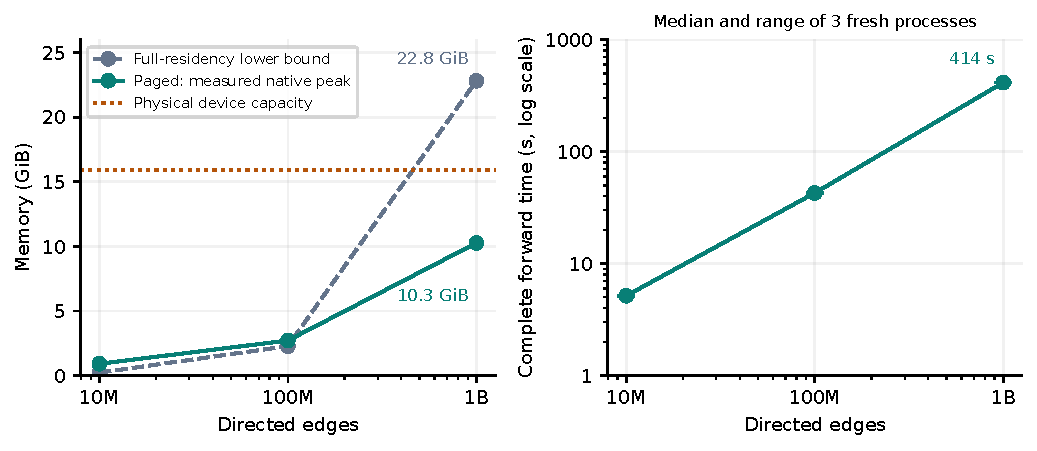
\includegraphics[width=\linewidth]{figures/billion-capacity.pdf}
\caption{One billion explicit edges on a single RTX 5070 Ti. Left: measured
native allocation peak versus the calculated full-residency lower bound, not
an executed resident baseline. Right: median and range of three complete
forward calls in fresh processes, including host staging and output assembly.}
\label{fig:billion}
\end{figure}
All nine trials complete with zero elementwise error. At one billion edges, the median forward takes 414.25 s (range 411.36--415.61 s). The maximum native GPU allocation peak across trials is 10.27 GiB, including the 7.45 GiB output; forward process peak RSS is 8.83 GiB. The maximum sampled whole-device usage is 13.25 GiB, including existing services and runtime pools; one-second sampling is not an exact physical peak. Each trial checks all two billion FP32 output values outside the forward timing interval.

\FloatBarrier

This evaluates forward capacity, not a speedup over an executable billion-edge
resident baseline, training throughput, GPUDirect Storage or cold-NVMe bandwidth.
The workload fits host RAM, and the output remains on the GPU. Recurrent
execution under a controlled smaller budget is evaluated separately in
Appendix~\ref{app:recurrent}; it is not extrapolated to billion-edge recurrence.
\FloatBarrier



\subsection{Illustrative archived CSR measurements}
Table~\ref{tab:weighted} retains every registered hot-cache weighted-aggregation
configuration for a fixed pair: \code{tiga.prepared\_auto} and
\code{torch.sparse.mm}. These measurements are attributed to the archived RTX
5070 Ti suite, not to a new experiment for this draft. Values are FP32 with
131,072 nodes; index width and feature count are listed separately. Topology
distributions and locality vary. Preparation, first compilation and graph
construction are outside the candidate's prepared timing boundary.

\begin{table}[ht]
\centering\small
\begin{tabular}{lllrrrr}
\toprule
Topology & Locality & Index & F & Tiga & Torch & Ratio \\
\midrule
regular & local & i64 & 1 & 0.020 & 0.047 & 2.31$\times$ \\
regular & local & i64 & 16 & 0.025 & 0.232 & 9.19$\times$ \\
regular & local & i64 & 64 & 0.100 & 0.275 & 2.76$\times$ \\
irregular & random & i32 & 16 & 0.057 & 0.263 & 4.63$\times$ \\
irregular & random & i32 & 64 & 0.206 & 0.400 & 1.94$\times$ \\
powerlaw & local & i32 & 1 & 0.020 & 0.041 & 2.00$\times$ \\
powerlaw & local & i64 & 1 & 0.023 & 0.038 & 1.65$\times$ \\
powerlaw & random & i32 & 1 & 0.054 & 0.070 & 1.30$\times$ \\
powerlaw & random & i64 & 1 & 0.054 & 0.071 & 1.32$\times$ \\
lognormal & random & i32 & 1 & 0.054 & 0.071 & 1.31$\times$ \\
exponential & random & i32 & 1 & 0.055 & 0.071 & 1.29$\times$ \\
\bottomrule
\end{tabular}

\caption{Historical hot-cache neighbor aggregation, milliseconds. All 11
registered topology/feature configurations for the fixed provider pair are shown.
This is not end-to-end latency of today's ordinary Torch call.}
\label{tab:weighted}
\end{table}

The table illustrates sensitivity to relation structure and feature width, not a
framework ranking. The broader suite also contains cold-data-cache and nonprepared
paths, with different boundaries and relative outcomes. ``Cold cache'' here means
perturbed data-cache contents, not first-time JIT compilation. PyG has fused sparse
aggregation paths as well as gather--scatter; measuring one particular PyG operator
cannot support a claim about the entire framework.

\subsection{Workload coverage and remaining experiments}
\begin{table}[ht]
\centering\small
\begin{tabularx}{\linewidth}{l Y Y}
\toprule
Question & Evidence in this report & What is not measured here \\
\midrule
CSR forward scaling & Fresh 4-size, 2-width GPU curves & Complete GNN training or arbitrary degree skew \\
Graph capacity & Billion-edge CUDA forward beyond full-residency GPU capacity; controlled-budget CPU/CUDA checks & Beyond-host-RAM graphs, billion-edge recurrence and CUDA paged backward \\
Topology sensitivity & All 11 historical matched hot CSR configurations & New timings for every archived topology \\
Edge-NN forward/VJP & Archived suite and separate correctness gates & New whole-training scaling in this revision \\
Attention / dynamic relations & Existing exact/pruned and builder benchmarks in the implementation archive & One universal speedup across these different contracts \\
Multi-device execution & Two-host TCP scaling; two-host NCCL forward/VJP gate & NCCL/RCCL scaling and device-profiler overlap \\
\bottomrule
\end{tabularx}
\caption{A benchmark coverage map prevents a small set of curves from standing
in for all features of the project. Unmeasured claims remain unmeasured.}
\end{table}

\subsection{Reproducing and extending the evidence}
The paper's export script verifies input checksums, matches dimensions and
providers, and derives table entries from raw JSON. Its generated provenance lists
the files and hashes used. A missing or ambiguous row fails generation rather
than selecting an arbitrary fastest result. The checked-in table permits a
standalone PDF build; regenerating it requires the implementation archive.
The new \code{tools/build\_results.py} imports fresh raw samples, validates every
configuration, checks the IR snapshots against the compiler, and generates all
four scaling figures. Its data index records input and benchmark-source hashes.
Run provenance includes exact commands; the paper README gives the reproduction
workflow. The billion-edge validator additionally checks all nine independent
trials, complete elementwise oracle coverage, source identity, capacity arithmetic
and allocation limits before generating its figure. Exploratory trials do not
enter the reported curves.

Fresh release experiments must bind to a clean source revision and record
hardware, driver, provider versions, seed, effective arguments, warmup, sample
order, synchronization and timing boundaries. Include numerical correctness and
gradient checks before timing. Separate first-call latency, warm execution,
preparation and transfers. The implementation's \code{tools/run\_benchmark.py}
records command/environment/source information for new runs. Historical metadata
gaps remain disclosed until replaced by fresh measurements.

Independent validation should also cover repeated backward after parameter
updates, non-contiguous layouts, empty rows, isolated entities, duplicates,
malformed snapshots, unsupported combinations and multi-rank failure handling.
Clean installed-wheel tests must run outside the source checkout, without compiler
path overrides. Passing an editable-source test can otherwise conceal missing
wheel libraries. The base installation must be tested without Torch, not merely
with Torch present but unused.
